As we mentioned in previous sections, models that estimate human pose, particularly models that estimate 2D poses from a single image, require above-average hardware. These models can be loaded on the CPU but the speed that the model needs to run the estimation is about 0.2-0.3 frames per second in Intel Core i7-7700HQ (2.8GHz) which is considered an above-average CPU. On the other hand, having a GPU with at least 2 GB VRAM (that is the minimum allocated space that the models need to be loaded), the speed that the model needs to run the estimation is about 4-5 frames per second in NIVIDIA GeForce GTX 1050 which also is considered an above-average GPU. The difference in speed is enormous, GPU is about 20 times faster than the CPU. The application was tested on a laptop, MSI GL72M 7RDX. During the run-time, the hardware of the laptop is shown in the figure from the application MSI DRAGON CENTER:

 \begin{figure}[h]
	\centering
	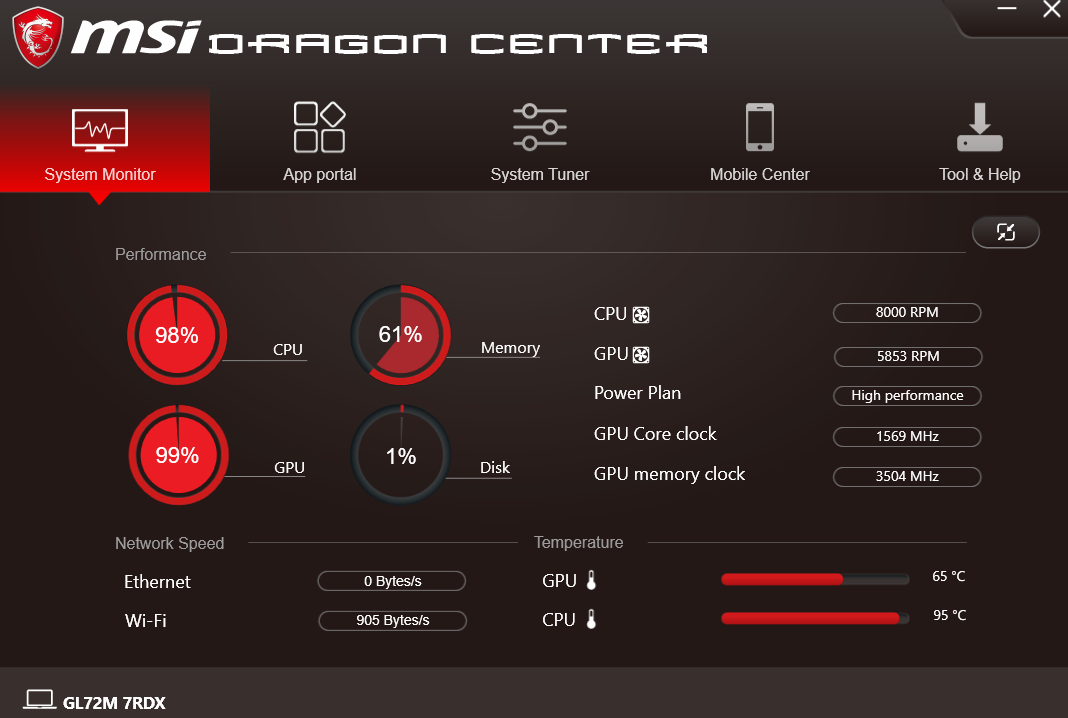
\includegraphics[width=1\textwidth]{figures/Requirements/Perfomance.png}
	\captionsetup{labelformat=empty}
	\caption{ MSI GL72M 7RDX performance stats}
\end{figure}